\section {Capacitor Modeling}

Many designers have a need to simulate the response of the individual components in their systems to impulse and steady state inputs. When dealing with passive electronic components, the device is typically modeled as a combination of various resitors, capacitors, and inductors. The model chosen is often due to either the required accuracy or a specific characteristic of the component that needs to be modeled. When characterizing a new component, the complex frequency response is recorded and then fit to a model. In this section, a progression of regression techniques will be evaluated for their ability to fit the measured frequency response of a capacitor to a polynomial equation. Then the accuracy of various capacitor models will be explored in regards to the fit. All models will attempt to fit the data from Figure: \ref{fig:exCapData}.

% This figure was generated by ./scripts/modeling/plot_ExCapData.m
\begin{figure}[ht!]
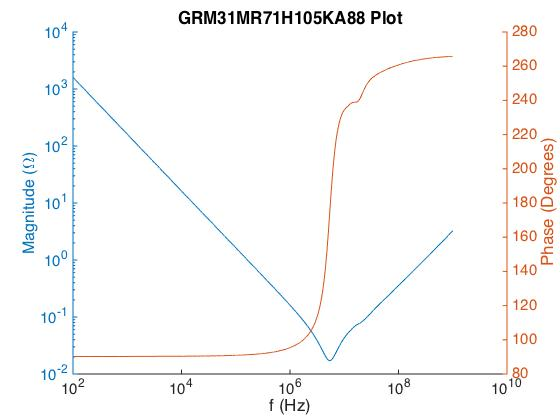
\includegraphics[keepaspectratio=true,width=6in]{./figures/modeling/exCapData.jpg}
\centering
\caption{GRM31MR71H105KA88 Capacitor Data}
\label{fig:exCapData}
\end{figure}



\subsection{Regression Analysis}
\label{sec:RegressionAnalysis}
\subsubsection{Basic LSE}
At its core, regression analysis is an optimization problem whose purpose is to fit the equation of a line to a data set. A commonly use regression analysis technique is called the Least Equares Estimate (LSE). It attempts to find a model which minimizes the squared error between an emperical set of data and itself.

The first step in applying a LSE is to choose the form of the equation that best represents the data. The equation of a line, Equation: \eqref{equ:ExLinEqu}, is chosen when only a simple linear fit is needed.
Then the squared error equation is generated, as in Equations: \eqref{equ:LSE_E2} \& \eqref{equ:LSE_E2b}.

\begin{equation}
\label{equ:ExLinEqu}
y = b_0 + b_1 x
\end{equation}

\begin{equation}
\label{equ:LSE_E2}
E^2 = \sum_{i=1}^{n} (y_i - y)^2
\end{equation}

\begin{equation}
\label{equ:LSE_E2b}
E^2 = \sum_{i=1}^{n} (y_i - (b_0 + b_1 x_i)^2
\end{equation}

In order to minimize the squared error over the data set, we need to take the partial derivate of Equation: \eqref{equ:LSE_E2b} with respect to each of the unknown parameters, the coefficients, seperately. While $b_0$ and $b_1$ will be constants in the final equation, they are treated as variables here until they are known. Conversely, all $x_i$ values are treated as constants. This results in Equations: \eqref{equ:LSE_PD1} \& \eqref{equ:LSE_PD2}.

\begin{equation}
\label{equ:LSE_PD1}
\frac{\partial E^2}{\partial b_0} = 0 = \sum_{i=1}^{n} (-2y_i +2b_0 + 2b_1 x_i)
\end{equation}

\begin{equation}
\label{equ:LSE_PD2}
\frac{\partial E^2}{\partial b_1} = 0 = \sum_{i=1}^{n} (-2y_i x_i +2b_0 x_i + 2b_1 x_i^2)
\end{equation}

Up to this point most LSE analyses follow the same basic path. But the rest of the steps depend upon the complexity of the model and solution techniques. The following steps in the basic LSE use transformations and substitutions to solve for the unknown variables. In our case, we can use Equations: \eqref{equ:avg} \& \eqref{equ:avgb} to remove the summation terms from the equation.

\begin{equation}
\label{equ:avg} 
\bar{y} = (\sum_{i=1}^{n} y_i) / n
\end{equation}

\begin{equation}
\label{equ:avgb} 
\sum_{i=1}^{n} y_i  = \bar{y}n
\end{equation}

This results in Equations: \eqref{equ:LSE_sol} \& \eqref{equ:LSE_solb} with solutions shown in Equations: \eqref{equ:LSE_solc} \& \eqref{equ:LSE_sold}. The empirical data is then used to find the values of $b_0$ and $b_1$. At this point, the line can be used to estimate new points on the plot or to compare against other data sets.

\begin{equation}
\label{equ:LSE_sol}
0 = \bar{y} - (b_0 + 2b_1 \bar{x})
\end{equation}

\begin{equation}
\label{equ:LSE_solb}
0 = \bar{xy} - (b_0 \bar{x} + 2b_1 \bar{x^2})
\end{equation}

\begin{equation}
\label{equ:LSE_solc}
b_0 = \bar{y} - b_1 \bar{x}
\end{equation}

\begin{equation}
\label{equ:LSE_sold}
b_1 = \frac{\bar{xy} - \bar{x}\bar{y}}{\bar{x^2} - \bar{x}^2}
\end{equation}

\subsubsection{Levy's Technique - Complex Curve Fitting}
While the basic LSE technique is sufficient for many circumstances, it is not directly applicable in situations where we need to fit a complex line, such as a transfer function. Levy \cite{levy} shows an extension of the simple LSE example that is valid for a genaric polynomial transfer function. This method is important because it not only allows for a complex-valued transfer functions, but it also prevents the nececcity of needing to rederive the system of equations for each new model. 

\begin{equation}
\label{equ:levy_Gs}
G(s) = \frac{A_0 + A_1 s + A_2 s^2 + ... + A_n s^n}{B_0 + B_1 s + B_2 s^2 + ... + B_n s^n}
~\cite{levy}[Eq.~3]
\end{equation}

Using Equation: \eqref{equ:levy_Gs} as the genaric model for the equation at hand, Levy shows that you can use Equations: \eqref{equ:Levy_L}, \eqref{equ:Levy_S}, \eqref{equ:Levy_T}, \& \eqref{equ:Levy_U} to simplify the series of partial derivates into a single matrix mtiplication equation shown in \eqref{equ:Levy_Ans}, \eqref{equ:Levy_M}, \eqref{equ:Levy_N}, \& \eqref{equ:Levy_C}.

\begin{equation}
\label{equ:Levy_L}
\lambda _h = \sum_{k=0}^{m} \omega _k ^h
~\cite{levy}[Eq.~15]
\end{equation}

\begin{equation}
\label{equ:Levy_S}
S_h = \sum_{k=0}^{m} \omega _k ^h R_k
~\cite{levy}[Eq.~16]
\end{equation}

\begin{equation}
\label{equ:Levy_T}
T_h = \sum_{k=0}^{m} \omega _k ^h I_k
~\cite{levy}[Eq.~17]
\end{equation}

\begin{equation}
\label{equ:Levy_U}
U_h = \sum_{k=0}^{m} \omega _k ^h (R_k ^2 + I_k ^2)
~\cite{levy}[Eq.~18]
\end{equation}

\begin{equation}
\label{equ:Levy_Ans}
MN = C
~\cite{levy}[Eq.~20]
\end{equation}

\setcounter{MaxMatrixCols}{12} % Allows each row of M to fit on one line
\begin{equation}
\label{equ:Levy_M}
M = 
\begin{bmatrix}
\lambda _0 & 0          & -\lambda _2 &  0           & \lambda _4  & \cdots &  T_1    & S_2    & -T_3   & -S_4   &  T_5    & \cdots \\
0          & \lambda _2 & 0           & -\lambda _4  & 0           & \cdots & -S_2    & T_3    &  S_4   & -T_5   & -S_6    & \cdots \\
\lambda _2 & 0          & -\lambda _4 &  0           & \lambda _6  & \cdots &  T_3    & S_4    & -T_5   & -S_6   &  T_7    & \cdots \\
0          & \lambda _4 & 0           & -\lambda _6  & 0           & \cdots & -S_4    & T_5    &  S_6   & -T_7   & -S_8    & \cdots \\

\vdots     & \vdots     &  \vdots     & \vdots       & \vdots      &        &  \vdots & \vdots & \vdots & \vdots &  \vdots &        \\ 
T_1        & -S_2       & -T_3        &  S_4         & T_5         & \cdots &  U_2    & 0      & -U_4   &  0     &  U_6    & \cdots \\
S_2        &  T_3       & -S_4        & -T_5         & S_6         & \cdots &  0      & U_4    &  0     & -U_6   &  0      & \cdots \\
T_3        & -S_4       & -T_5        &  S_6         & T_7         & \cdots &  U_4    & 0      & -U_6   &  0     &  U_8    & \cdots \\
\vdots     & \vdots     &  \vdots     & \vdots       & \vdots      & \vdots &  \vdots & \vdots & \vdots & \vdots &  \vdots &        \\ 
\end{bmatrix}
~\cite{levy}[Eq.~21a]
\end{equation}

\begin{multicols}{2}
\begin{equation}
\label{equ:Levy_N}
N = 
\begin{bmatrix}
A_0 \\
A_1 \\
A_2 \\
A_3 \\
\vdots \\
B_1 \\
B_2 \\
B_3 \\
\vdots
\end{bmatrix}
~\cite{levy}[Eq.~21b]
\end{equation}

\begin{equation}
\label{equ:Levy_C}
C = 
\begin{bmatrix}
S_0 \\
T_1 \\
S_2 \\
T_3 \\
\vdots \\
0   \\
U_2 \\
0   \\
\vdots
\end{bmatrix}
~\cite{levy}[Eq.~21c]
\end{equation}
\end{multicols}

Levy's technique works well for applications where there is a small dynamic frequency range and a small number of coefficients, but there a several problems with it.
The first problem is that for models with a wide bandwidth, the solution to Equation: \eqref{equ:Levy_Ans}, involves an ill-conditioned matrix. This means that the ratio of the "largest to smallest singular value in the singular value decomosition of a matrix is ... $>= log^{-1}$(input precision). In other words, it estimates a worse case loss of precision."
The second problem is that this technique favors the magnitude plot at the high frequency range. 

% Run /scripts/regression/run_levy_iter.m with NumDeg = 3, DenDeg = 3, and iterations = 1.
\begin{figure}[ht!]
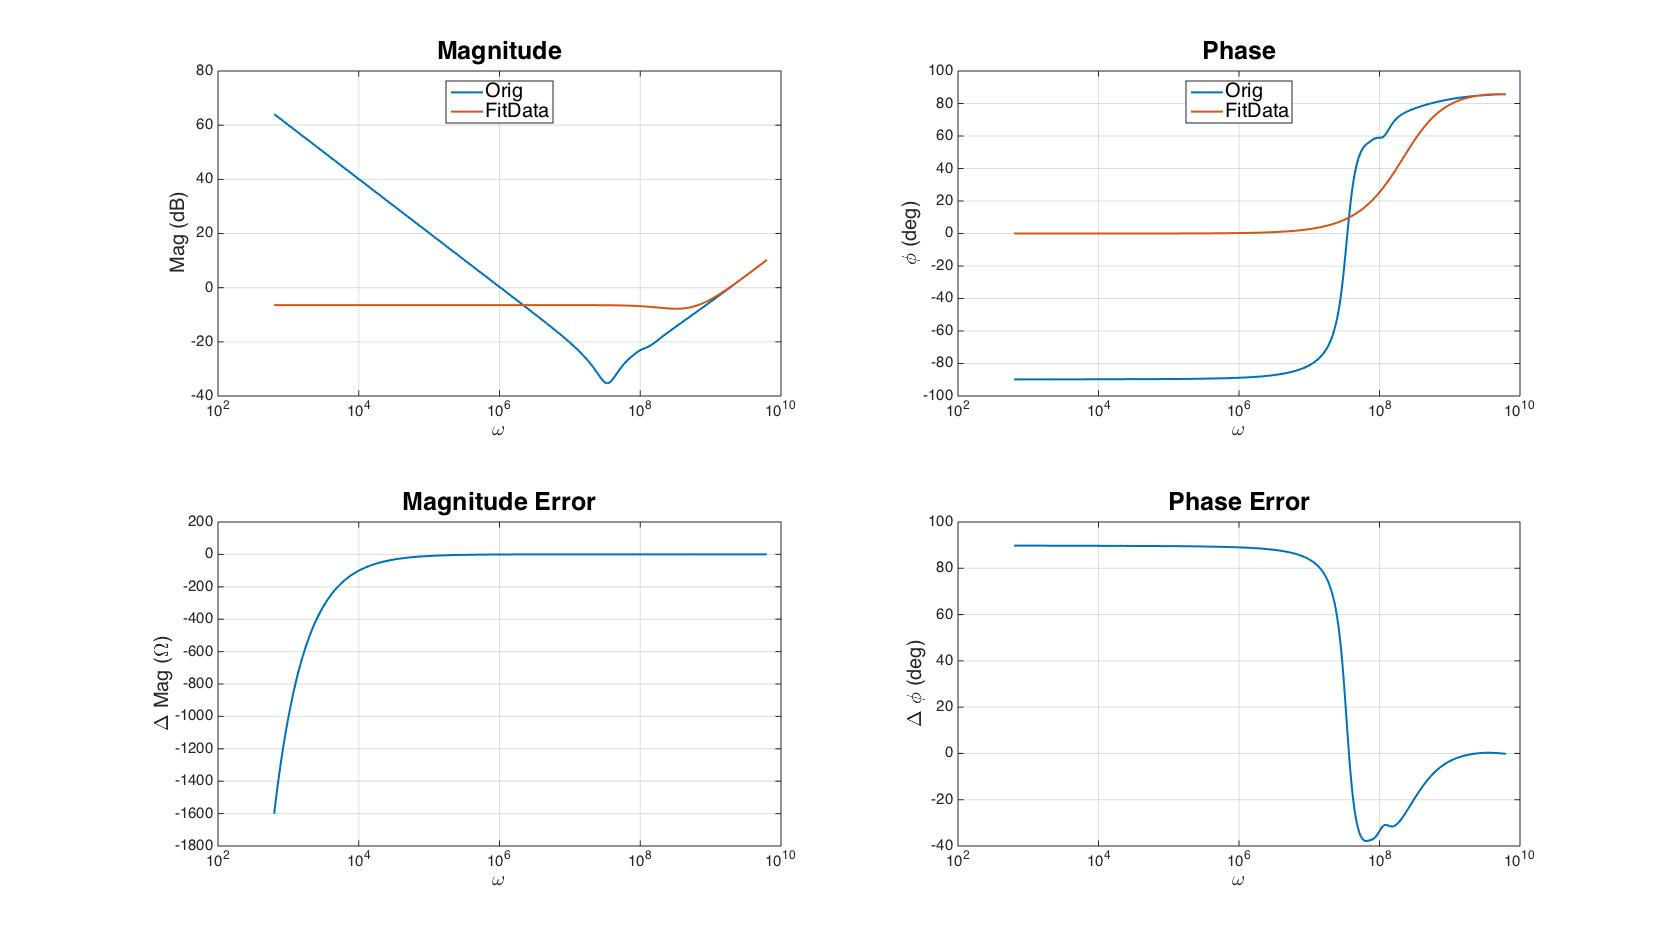
\includegraphics[keepaspectratio=true,width=6in]{./figures/regression/levy.jpg}
\centering
\caption{Levy's Technique}
\label{fig:levy}
\end{figure}



\subsubsection{Weighted LSE}
One improvement that can be made upon Levy's method is to iterate with a weighting function untill the error term is minimized\cite{levy_iter}. By multiplying Levy's error function by the weighting term in Equation: \eqref{equ:iter_Weight}, we get Equation: \eqref{equ:iter_Err}, which can be minimized to obtain a new system of equations.

\begin{equation}
\label{equ:iter_Weight}
W_{kL} = \frac{1}{|Q(jw_k)_{L-1}|^2}
~\cite{levy_iter}
\end{equation}

\begin{equation}
\label{equ:iter_Err}
E = \sum_{k=1}^{n} |\epsilon _k ^{'}|^2W_{kL}
~\cite{levy_iter}[Eq.~7]
\end{equation}

Equations \eqref{equ:Levy_Ans}, \eqref{equ:Levy_M}, \& \eqref{equ:Levy_N} are the same, with Equations \eqref{equ:Levy_L}, \eqref{equ:Levy_S}, \eqref{equ:Levy_T}, \& \eqref{equ:Levy_U} being replaced with Equations: \eqref{equ:Iter_L}, \eqref{equ:Iter_S}, \eqref{equ:Iter_T}, \& \eqref{equ:Iter_U}.
The $L$ subscript stands for the current iteration, while $L-1$ stands for the previous iteration.

\begin{equation}
\label{equ:Iter_L}
\lambda _h = \sum_{k=0}^{m} \omega _k ^hW_{kL}
~\cite{levy_iter}[Eq.~9]
\end{equation}

\begin{equation}
\label{equ:Iter_S}
S_h = \sum_{k=0}^{m} \omega _k ^h R_kW_{kL}
~\cite{levy_iter}[Eq.~10]
\end{equation}

\begin{equation}
\label{equ:Iter_T}
T_h = \sum_{k=0}^{m} \omega _k ^h I_kW_{kL}
~\cite{levy_iter}[Eq.~11]
\end{equation}

\begin{equation}
\label{equ:Iter_U}
U_h = \sum_{k=0}^{m} \omega _k ^h (R_k ^2 + I_k ^2)W_{kL}
~\cite{levy_iter}[Eq.~12]
\end{equation}


This particular iteration method is not gauranteed to converge. Looking at Figure: \ref{fig:levyIter_Err1}. The squared error of the magnitude and phase do not converge after a particular number of iterations. Furthermore, they do not reach their minimums at the same iteration. In order to select the desired iteration, the magnitude and phase squared plots are normalized as such $n = min(Emag/max(eMag) + Epha/max(ePha))$. The index of the minium of Figure: \ref{fig:levyIter_Err1} is selected as the best fit.

\begin{figure}[ht!]
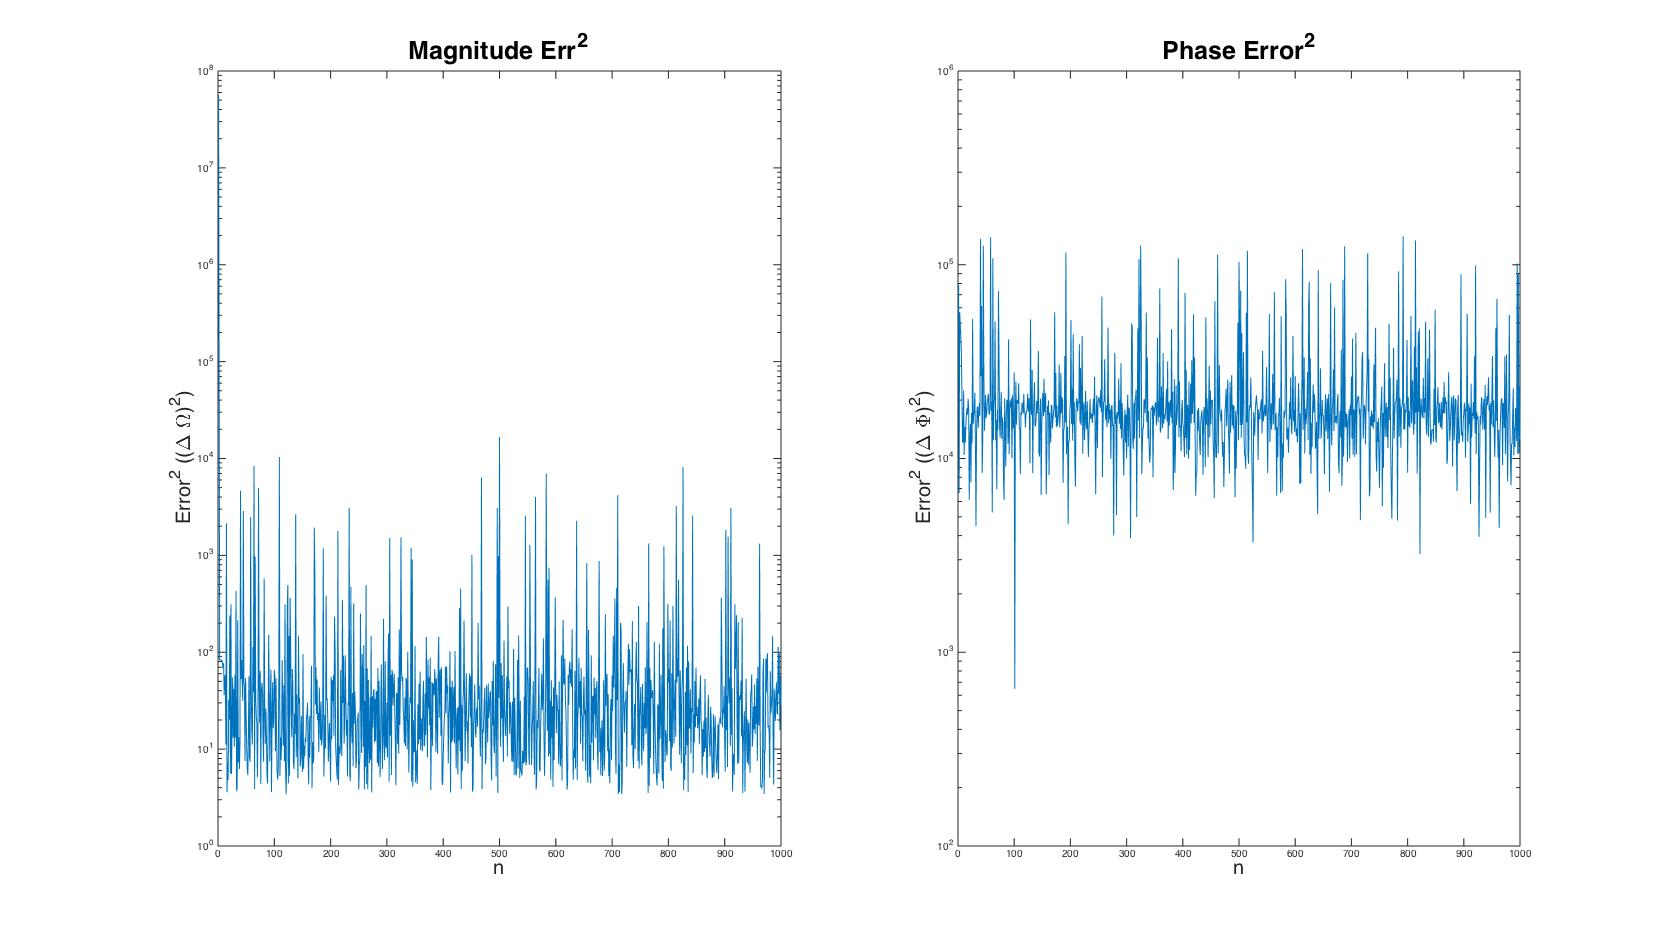
\includegraphics[keepaspectratio=true,width=6in]{./figures/modeling/levyIter_Err1.jpg}
\centering
\caption{LSE + Iteration -- Magnitude and Phase Error}
\label{fig:levyIter_Err1}
\end{figure}

% Run ./scripts/regression/run_levy_iter.m with numDeg = 7, denDeg = 7, and iterations = 100 to obtain this image.
\begin{figure}[ht!]
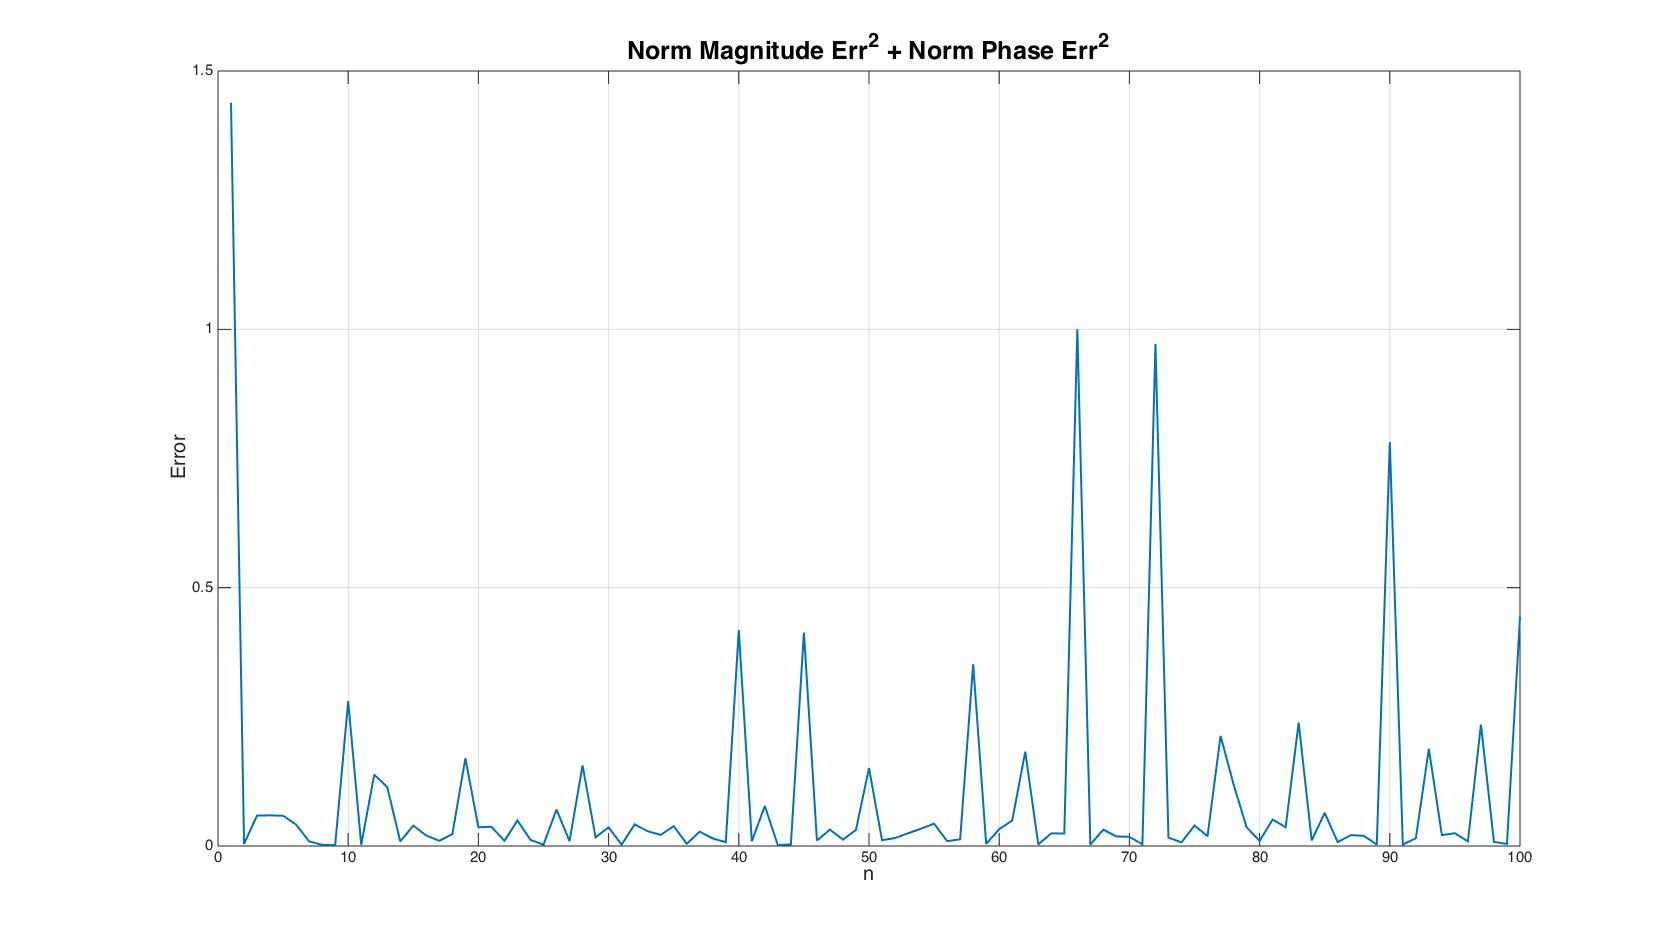
\includegraphics[keepaspectratio=true,width=6in]{./figures/regression/levyIter_Err2.jpg}
\centering
\caption{LSE + Iteration -- Combined Error}
\label{fig:levyIter_Err2}
\end{figure}



Figure: \ref{fig:levyIter} shows that this method can result in a much improved result over the Levy's original method, as sseen in Figure: \ref{fig:levy}.

\begin{figure}
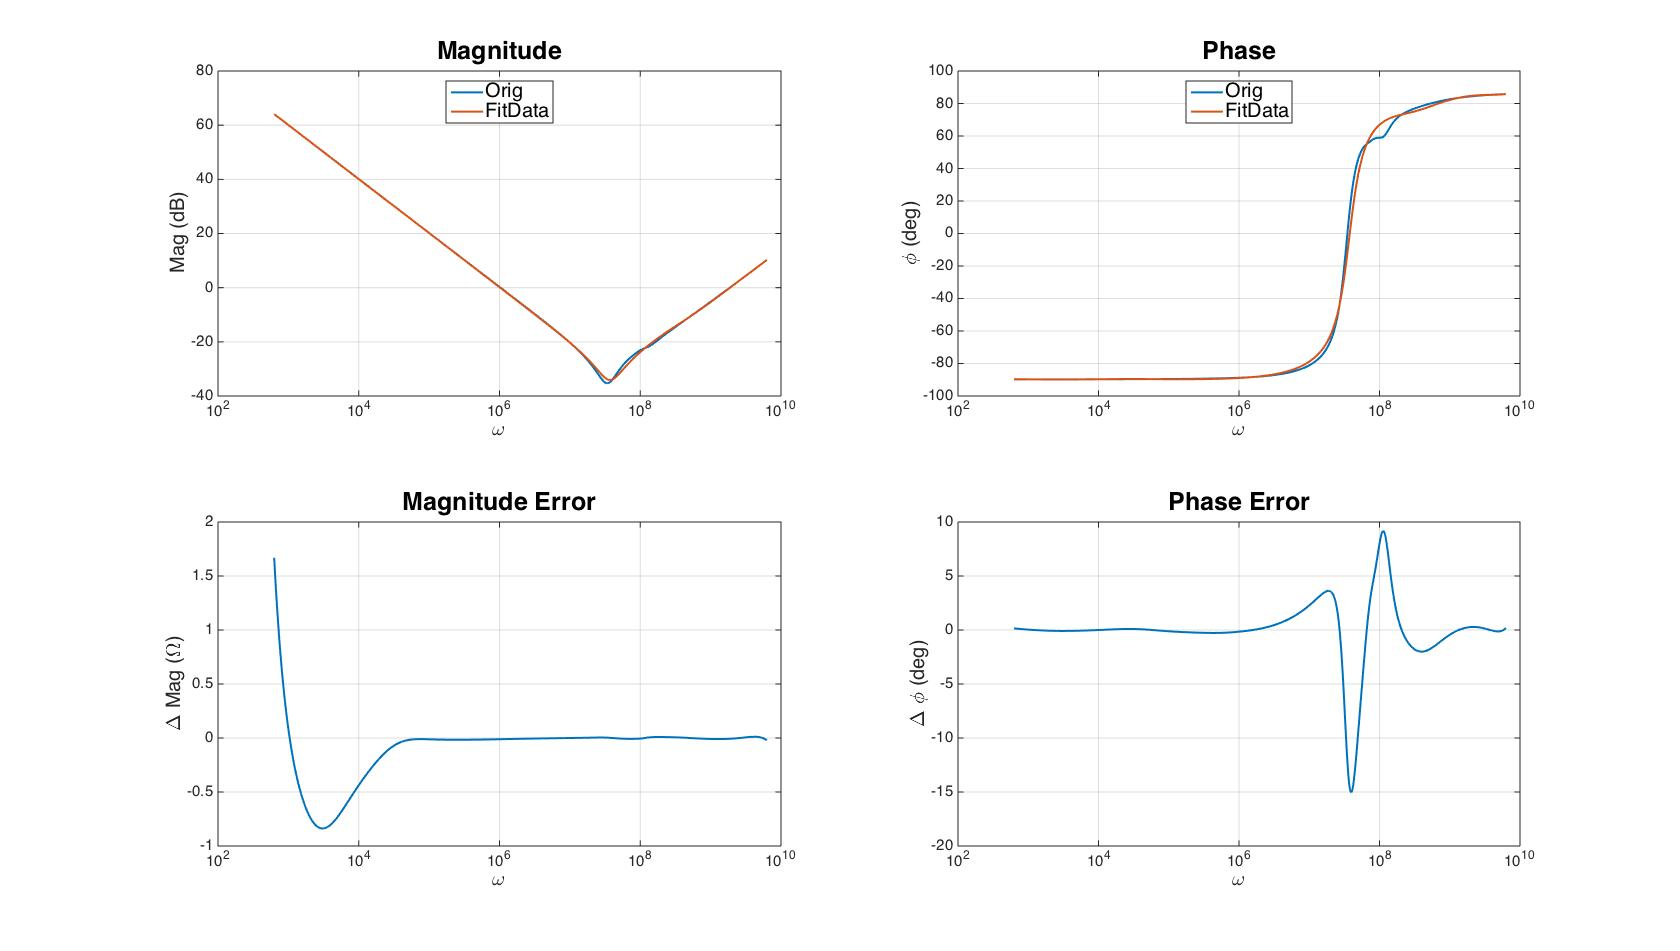
\includegraphics[keepaspectratio=true,width=6in]{./figures/modeling/levyIter.jpg}
\centering
\caption{LSE + Iteration}
\label{fig:levyIter}
\end{figure}



\subsection{Modeling}
This section will investigate several of the most common capacitor models. It will show how to fit them to a data set with Levy's method described in Section: \ref{sec:RegressionAnalysis}, and will describe their effectiveness and limitations in doing so.

\subsubsection{RLC}
\begin{figure}[ht!]
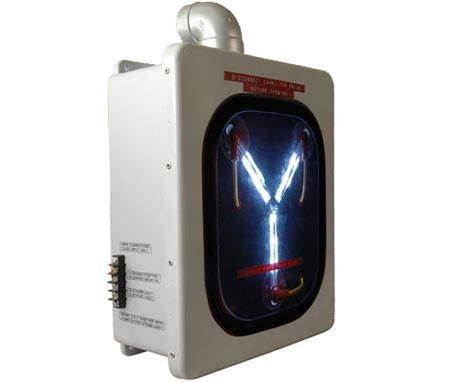
\includegraphics[keepaspectratio=true,width=2in]{./figures/regression/rlcModel.jpg}
\centering
\caption{RLC Model}
\label{fig:rlcModel}
\end{figure}


The RLC model, shown in Figue: \ref{fig:rlcModel}, is one of the simplest models used to describe a capacitor. It shows the basic low and high frequency characteristics, along with the capacitor's resonant point. Its impedance is described in Equations: \eqref{equ:rlc_Zs} \& \eqref{equ:rlc_Zs2}, but our method does not allow for any poles at the origin. In Equation: \eqref{equ:rlc_Zs3} we multiply by $s$ and fit the new equation to the data. At the end, we will divide by $s$ to get our final result. At this point out eqution is in the proper form and can be abstracted into Equation \eqref{equ:rlc_Zs4}.

\begin{equation}
\label{equ:rlc_Zs}
Z(s) = R + sL + \frac{1}{sC}
\end{equation}

\begin{equation}
\label{equ:rlc_Zs2}
Z(s) = \frac{1 + s(RC) + s^2 (LC)}{sC}
\end{equation}

\begin{equation}
\label{equ:rlc_Zs3}
Z_2(s) = Z(s) * s =  \frac{\frac{1}{C} + s(R) + s^2 (L)}{1}
\end{equation}

\begin{equation}
\label{equ:rlc_Zs4}
Z_2(s) = \frac{A_0 + A_1 s + A_2 s^2}{B_0 + B_1 s + B_2 s^2}
\end{equation}

For this model Equations: \eqref{equ:Levy_M}, \eqref{equ:Levy_N}, \& \eqref{equ:Levy_C} simplify down to Equations: \eqref{equ:rlc_M}, \eqref{equ:rlc_N}, \& \eqref{equ:rlc_C}.

\begin{equation}
\label{equ:rlc_M}
M = 
\begin{bmatrix}
\lambda _0 & 0          & -\lambda _2 &  T_1    & S_2 \\
0          & \lambda _2 & 0           & -S_2    & T_3 \\
\lambda _2 & 0          & -\lambda _4 &  T_3    & S_4 \\
T_1        & -S_2       & -T_3        &  U_2    & 0   \\
S_2        &  T_3       & -S_4        &  0      & U_4
\end{bmatrix}
\end{equation}

\begin{multicols}{2}
\begin{equation}
\label{equ:rlc_N}
N = 
\begin{bmatrix}
A_0 \\
A_1 \\
A_2 \\
B_1 \\
B_2
\end{bmatrix}
\end{equation}

\begin{equation}
\label{equ:rlc_C}
C = 
\begin{bmatrix}
S_0 \\
T_1 \\
S_2 \\
0   \\
U_2
\end{bmatrix}
\end{equation}
\end{multicols}

Fitting this model to the data shown in Figure:

